\section{Xây dựng mô hình dự đoán}

\subsection{Tiền xử lý và chia tập huấn luyện}
\hspace{17pt}Trước khi đưa dữ liệu vào huấn luyện các mô hình học máy, một bước đánh giá cực kỳ quan trọng là phải kiểm chứng xem tập dữ liệu kiểm thử (Test set - 20\%) có mang tính đại diện chính xác cho tập dữ liệu huấn luyện (Train set - 80\%) hay không. Nếu phân phối của hai tập này bị lệch (Data Drift), kết quả đánh giá mô hình sẽ không còn phản ánh đúng năng lực dự đoán thực tế.

\hspace{17pt}Đầu tiên, nhóm tiến hành kiểm tra sự phân bổ của biến mục tiêu (\texttt{Potability}) ở cả hai tập:
\begin{figure}[H]
    \centering
    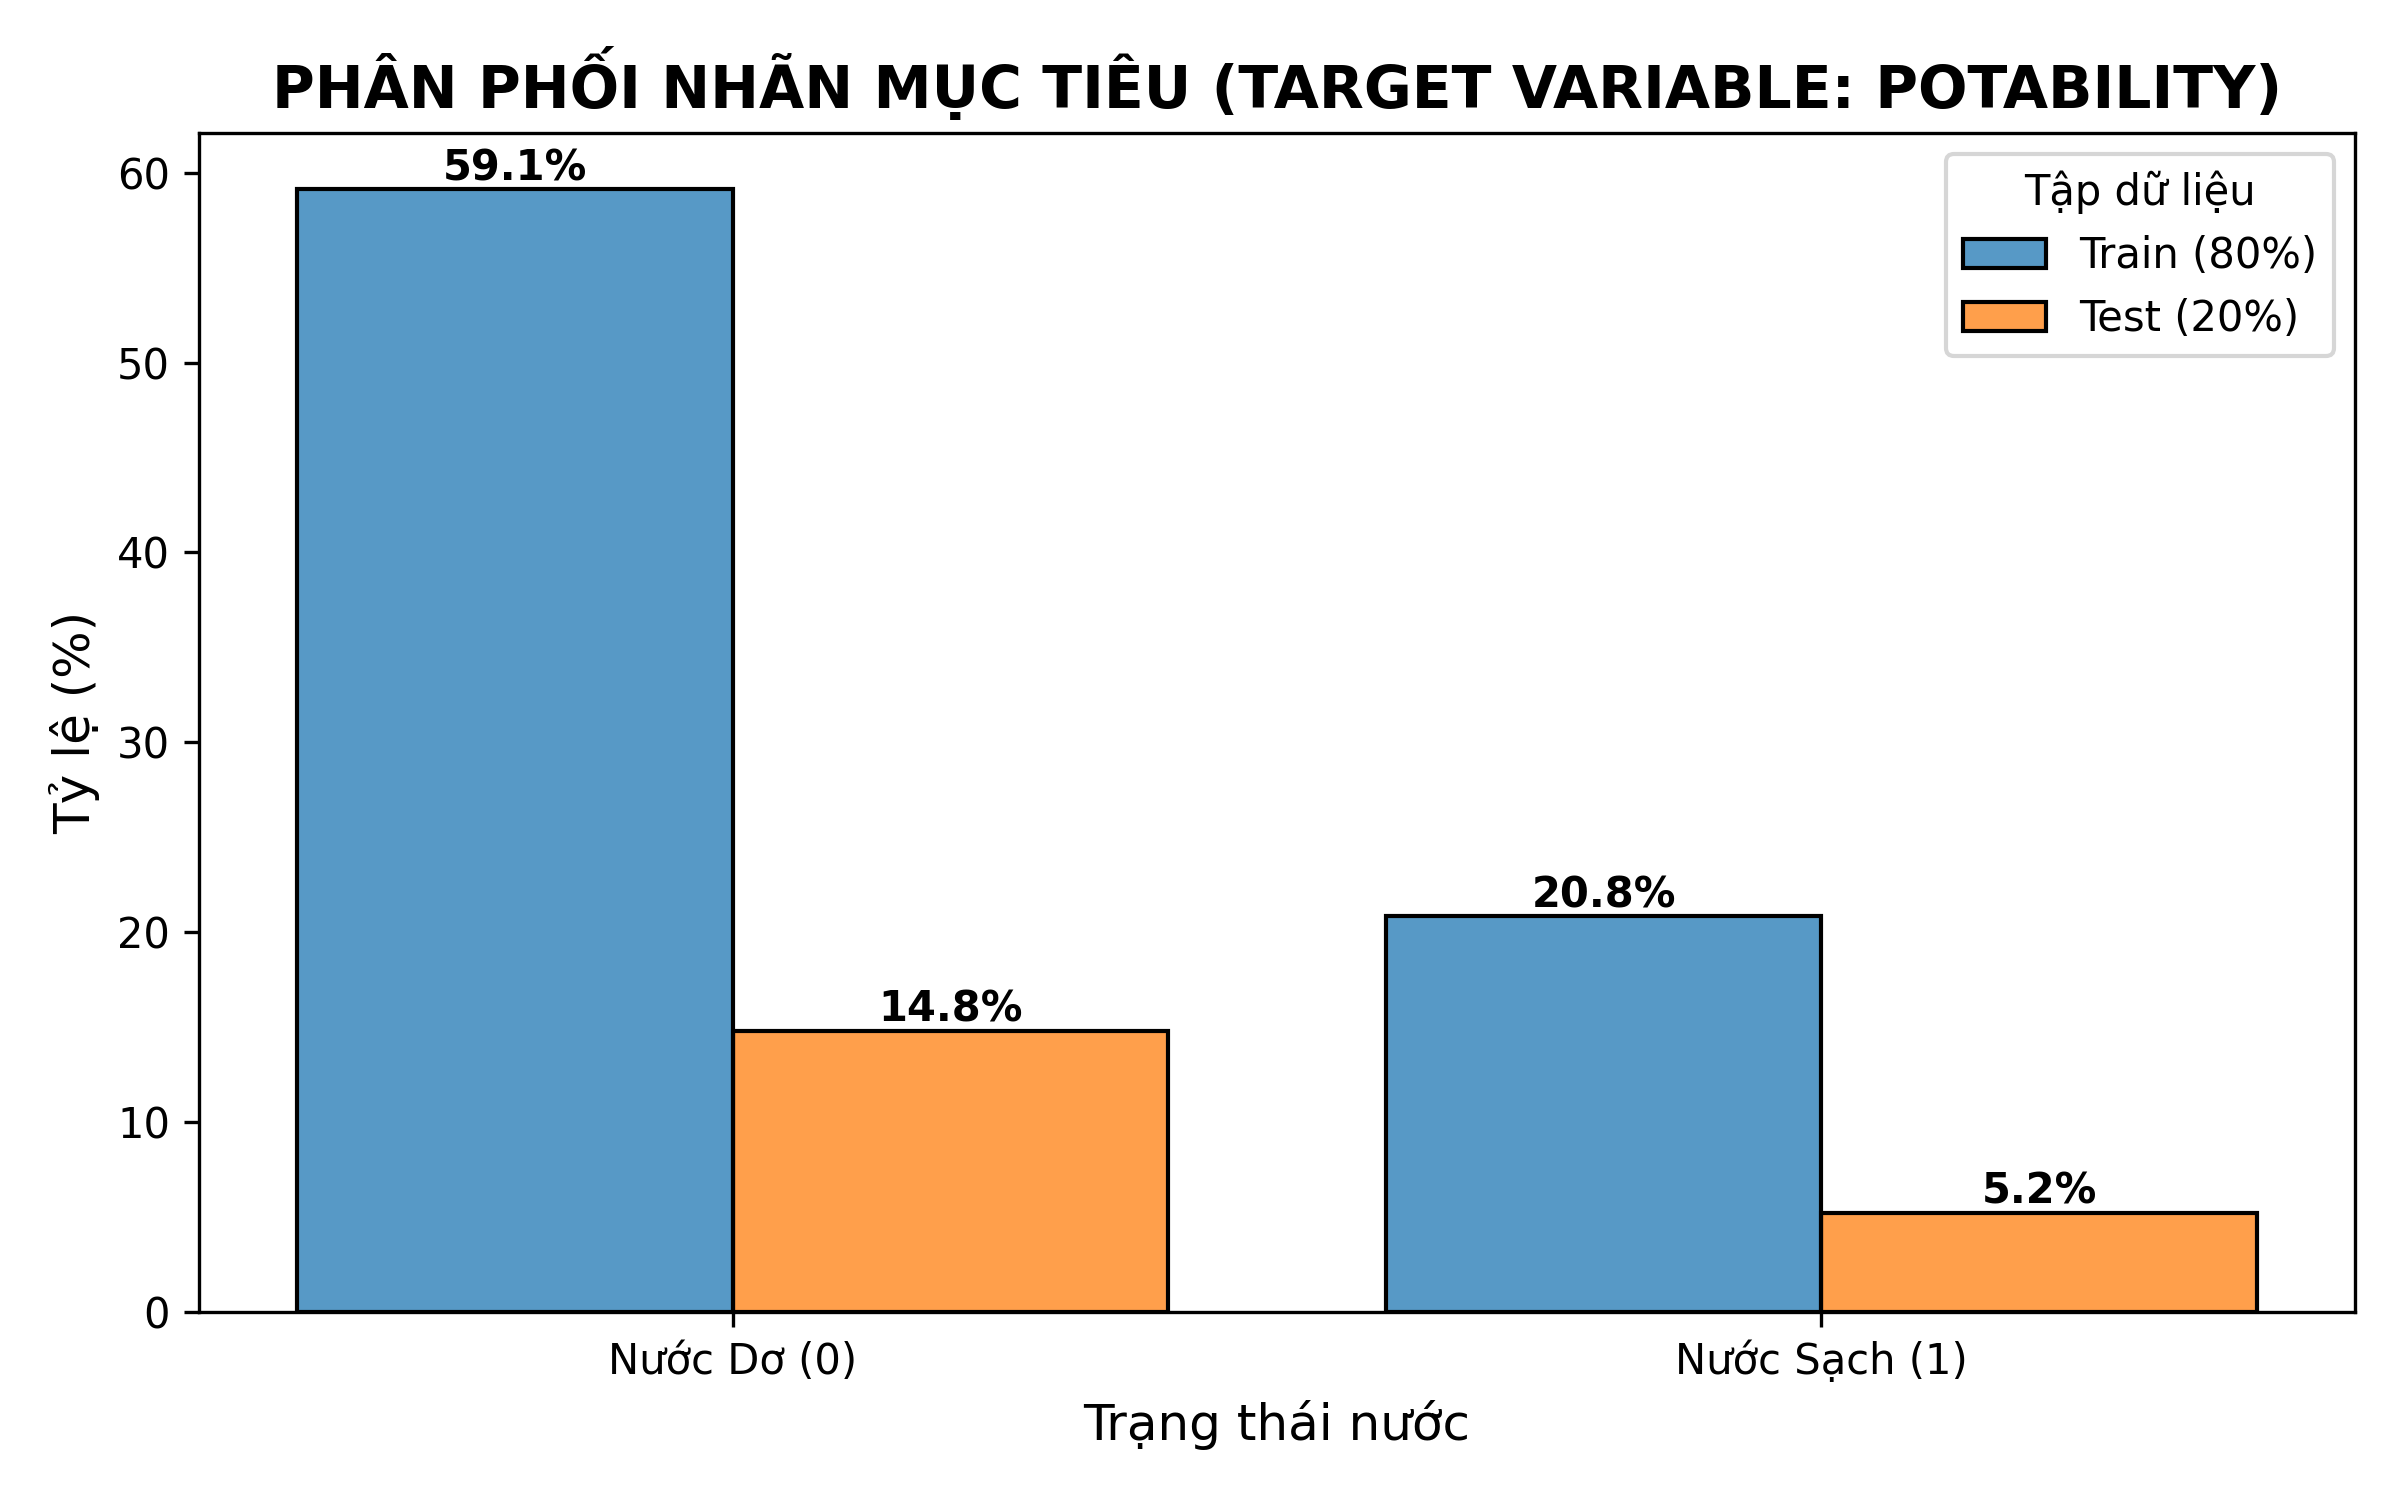
\includegraphics[width=1.0\linewidth]{IMAGE-MODELS/Histogram_Target_Plot.png}
    \caption{
    Phân phối nhãn mục tiêu (Potability) trên tập Train và Test}
    \label{fig:placeholder}
\end{figure}

\hspace{17pt}Tiếp theo, nhóm tiến hành kiểm tra cấu trúc phân phối của toàn bộ các đặc trưng hóa lý (Features) đầu vào:
\begin{figure}[H]
    \centering
    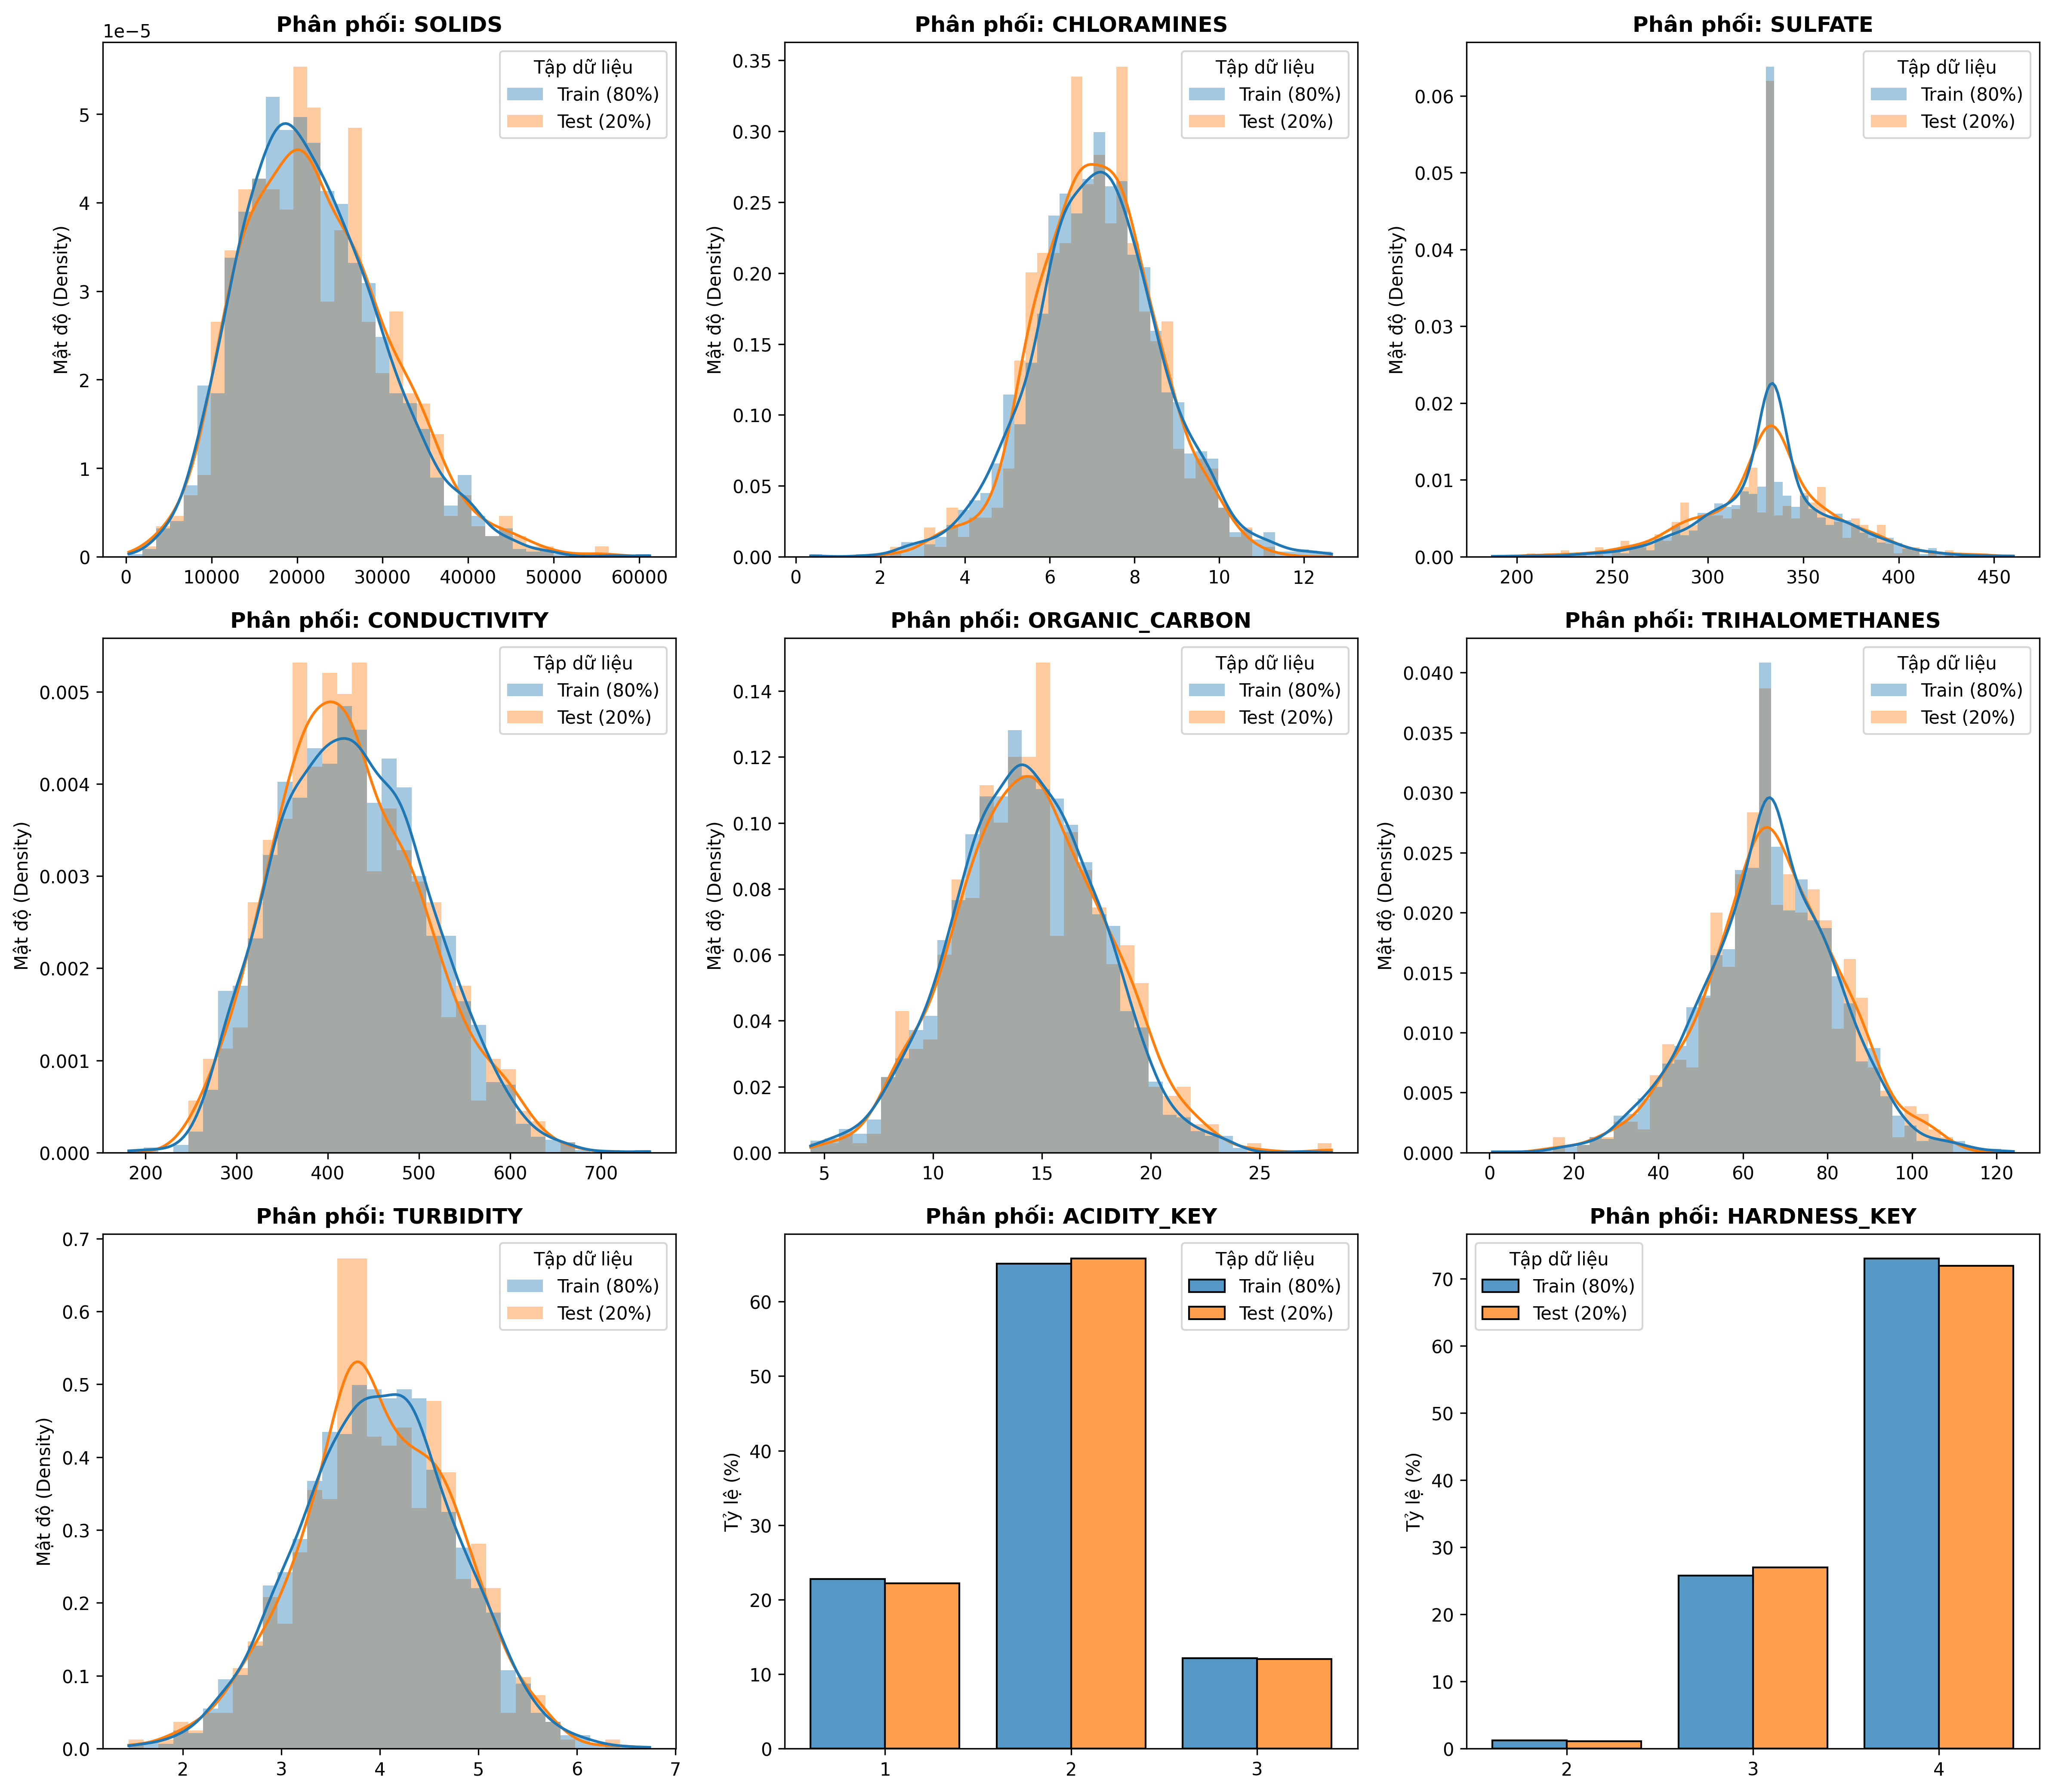
\includegraphics[width=1.0\linewidth]{IMAGE-MODELS/Histogram_Features_Plot.png}
    \caption{So sánh phân phối của các đặc trưng hóa lý trên tập Train và Test}
    \label{fig:features_dist}
\end{figure}
\hspace{17pt}Biểu đồ Hình \ref{fig:features_dist} cung cấp cái nhìn tổng quan về mật độ phân phối của các đặc trưng:
\begin{itemize}
    \item \textbf{Sự đồng nhất về phân phối:} Đường cong mật độ (KDE) của tập Train (màu xanh) và tập Test (màu cam) gần như chồng khít lên nhau ở tất cả các biến liên tục như \texttt{Solids}, \texttt{Chloramines}, hay \texttt{Conductivity}. Các biến rời rạc (\texttt{Acidity\_key}, \texttt{Hardness\_key}) cũng bảo toàn hoàn toàn cấu trúc tỷ lệ. Điều này khẳng định tập Test chứa các mẫu ngẫu nhiên và mang tính đại diện cực kỳ tốt cho tập Train.
    \item \textbf{Dấu vết của quá trình ETL (Imputation Artifact):} Điểm đáng chú ý là đỉnh nhọn bất thường xuyên thủng đường phân phối chuẩn tại biểu đồ \texttt{Sulfate} và \texttt{Trihalomethanes}. Đây không phải là lỗi dữ liệu, mà chính là minh chứng trực quan cho bước ETL Điền khuyết (Imputation) bằng giá trị trung bình/trung vị đã thực hiện ở giai đoạn trước đối với các giá trị \texttt{NaN}. Mặc dù tạo ra đỉnh nhọn, nhưng đỉnh này xuất hiện đồng đều ở cả tập Train và Test, đảm bảo tính nhất quán của dữ liệu.
\end{itemize}

\hspace{17pt}Với nền tảng dữ liệu đã được làm sạch, chuẩn hóa và phân tách đồng nhất, hệ thống đã hoàn toàn sẵn sàng cho quá trình huấn luyện và tối ưu siêu tham số các mô hình học máy.
Quá trình tiền xử lý đóng vai trò quyết định trong việc loại bỏ nhiễu và nâng cao chất lượng dữ liệu trước khi đưa vào mô hình học máy. Dữ liệu đầu vào được trích xuất trực tiếp từ kho dữ liệu (bảng \textit{fact\_water\_sample}) và đi qua các bước xử lý sau:

\begin{itemize}
    \item \textbf{Lựa chọn đặc trưng:} Lựa chọn các biến độc lập quan trọng bao gồm: \textit{solids, chloramines, sulfate, conductivity, organic\_carbon, trihalomethanes, turbidity}. Riêng hai đặc trưng \textit{pH} và \textit{hardness} được sử dụng dưới dạng đã được rời rạc hóa (binning) thành \textit{acidity\_key} và \textit{hardness\_key} để tối ưu khả năng phân loại của mô hình.
    
    \item \textbf{Làm sạch dữ liệu theo logic thực tế:} Nhằm loại bỏ các điểm dữ liệu phi thực tế. Dù có nhãn uống được (\textit{$Portability = 1$}), nhưng các chỉ số hóa lý lại ở mức độc hại. Các điều kiện lọc sau được áp dụng để xóa bỏ các bản ghi lỗi:
    \begin{itemize}
        \item Nước có tính axit mạnh ($pH<6.5$) hoặc kiềm mạnh ($pH> 8.5$).
        \item Nồng độ Sulfate vượt ngưỡng an toàn ($>400$).
        \item Tổng chất rắn hòa tan (Solids) quá cao ($>40000$), biểu hiện của nước quá mặn hoặc bị ô nhiễm nghiêm trọng.
        \item Độ đục (Turbidity) ở mức ngầu bùn ($>7$).
    \end{itemize}
    
    \item \textbf{Chia tập dữ liệu huấn luyện và kiểm thử:} Dữ liệu sau khi làm sạch được chia thành tập huấn luyện (80\%) và tập kiểm thử (20\%). Kỹ thuật phân tầng (\textit{stratify}) được áp dụng dựa trên nhãn mục tiêu nhằm đảm bảo tỷ lệ phân bố giữa lớp an toàn và không an toàn được giữ nguyên ở cả hai tập, hạn chế tối đa sự mất cân bằng lớp.
    
    \item \textbf{Chuẩn hóa dữ liệu (Data Scaling):} Sử dụng \textit{StandardScaler} để đưa các đặc trưng về cùng một dải phân phối chuẩn (trung bình bằng 0 và phương sai bằng 1). Quá trình fit\_transform được thực hiện trên tập huấn luyện và sau đó transform trên tập kiểm thử. Việc chuẩn hóa này là yêu cầu bắt buộc để các thuật toán dựa trên khoảng cách (như SVM) không bị sai lệch bởi sự chênh lệch đơn vị đo.
\end{itemize}

\subsection{Phương thức đánh giá mô hình}
Để đánh giá hiệu suất của các mô hình phân lớp một cách toàn diện, thay vì chỉ dựa vào độ chính xác (Accuracy), nghiên cứu tập trung vào việc đánh giá khả năng nhận diện đúng mẫu nước an toàn (Lớp 1). Các độ đo chính được sử dụng bao gồm: Precision (Độ chính xác dự đoán), Recall (Độ bao phủ) và F1-Score (Trung bình điều hòa giữa Precision và Recall).

Một điểm đáng chú ý trong phương pháp đánh giá của nghiên cứu này là kỹ thuật \textbf{Quét ngưỡng quyết định (Threshold Scanning)}. Thay vì sử dụng ngưỡng mặc định là 0.5 để phân lớp, hệ thống thực hiện quét liên tục các ngưỡng xác suất (từ 0.5 đến 0.8 với bước nhảy 0.02) dựa trên kết quả \textit{predict\_proba}. Kỹ thuật này giúp tìm ra ngưỡng cắt tối ưu nhất, cho phép cân bằng linh hoạt giữa việc không bỏ sót nguồn nước an toàn (Recall cao) và đảm bảo không uống nhầm nước độc hại (Precision cao). 

Quá trình hiện thực kỹ thuật quét ngưỡng được thể hiện chi tiết trong Đoạn mã \ref{lst:threshold_scanning}.

\begin{lstlisting}[language=Python, caption={Thuật toán quét ngưỡng quyết định (Threshold Scanning)}, label={lst:threshold_scanning}]
thresholds = np.arange(0.5, 0.8, 0.02)
for name, model in models.items():
    test_data = X_test_scaled if name == "SVM" else X_test
    y_proba = model.predict_proba(test_data)[:, 1]
    for th in thresholds:
        th = round(th, 2)
        y_pred_custom = (y_proba >= th).astype(int)
        
        report = classification_report(y_test, y_pred_custom, 
                                       output_dict=True, zero_division=0)
        
        p1 = report['1']['precision']
        r1 = report['1']['recall']
        f1 = report['1']['f1-score']
        acc = report['accuracy']
\end{lstlisting}
\subsection{Hiện thực mô hình dự đoán}
Nghiên cứu tiến hành cài đặt và huấn luyện ba thuật toán học máy phổ biến và mạnh mẽ nhất cho bài toán phân lớp:
\begin{enumerate}
    \item \textbf{Random Forest:} Thuật toán học tập hợp (Ensemble Learning) dựa trên cây quyết định, được thiết lập với 100 cây ước lượng (\textit{n\_estimators=100}). Thuật toán này có khả năng tự xử lý tốt các đặc trưng phi tuyến và không yêu cầu khắt khe về việc chuẩn hóa dữ liệu.
    \item \textbf{XGBoost (Extreme Gradient Boosting):} Mô hình Boosting mạnh mẽ với 100 bộ ước lượng, giúp tối ưu hóa hàm mất mát thông qua việc học tuần tự từ các sai số của các cây quyết định trước đó.
    \item \textbf{Support Vector Machine (SVM):} Được cấu hình với hàm nhân phi tuyến RBF (\textit{kernel='rbf'}) để xử lý không gian dữ liệu phức tạp và bật tính năng tính toán xác suất (\textit{probability=True}) phục vụ cho bước quét ngưỡng. Mô hình này được huấn luyện trực tiếp trên tập dữ liệu đã qua chuẩn hóa (\textit{X\_train\_scaled}).
\end{enumerate}

Thay vì sử dụng các tham số mặc định của thư viện, nghiên cứu áp dụng kỹ thuật \texttt{RandomizedSearchCV} với kiểm chứng chéo 5 nếp gấp (5-fold CV) để tự động dò tìm tổ hợp siêu tham số tối ưu nhất cho Random Forest và XGBoost. Riêng mô hình SVM được thiết lập cấu hình tĩnh do đặc thù thuật toán đòi hỏi chi phí tính toán phần cứng quá lớn.

\hspace{17pt}Để thực hiện việc dò tìm, nhóm đã định nghĩa một không gian siêu tham số (Hyperparameter Grid) bao gồm các tổ hợp giá trị tiềm năng nhất, kết hợp với danh sách các đặc trưng đầu vào và dải ngưỡng quét (Threshold Sweep). Toàn bộ được cấu hình tập trung và quản lý độc lập như sau:

\begin{lstlisting}[language=Python, caption=Cấu hình đặc trưng và không gian siêu tham số cho các mô hình]
import numpy as np

# 1. Cau hinh Data (Features)
FEATURES_TO_USE = [
    'solids', 'chloramines', 'sulfate', 'conductivity',
    'organic_carbon', 'trihalomethanes', 'turbidity',
    'acidity_key', 'hardness_key'  
]

# 2. Khong gian Sieu tham so (Hyperparameter Grids)
RF_PARAMS = {
    'n_estimators': [100, 200, 300, 500],
    'max_depth': [None, 10, 20, 30], # Do sau toi da cua cay
    'min_samples_split': [2, 5, 10], # So mau toi thieu de tach nhanh
    'random_state': [42],
    'class_weight': [None, 'balanced'] 
}

XGB_PARAMS = {
    'n_estimators': [100, 200, 300],
    'learning_rate': [0.01, 0.1, 0.2],
    'max_depth': [3, 5, 7],
    'subsample': [0.8, 1.0]
}

# Tham so tinh cho SVM
SVM_PARAMS = {
    'kernel': 'rbf',
    'probability': True,
    'random_state': 42
}

THRESHOLDS_SWEEP = np.arange(0.5, 0.8, 0.05) 
\end{lstlisting}
Sau khi các mô hình hoàn tất quá trình huấn luyện và quét ngưỡng để đối chiếu hiệu suất, các mô hình đạt kết quả tốt nhất (bao gồm Random Forest và SVM) cùng với bộ chuẩn hóa dữ liệu (Scaler) được đóng gói và xuất ra dưới định dạng tệp \textit{.pkl} thông qua thư viện \textit{joblib}. Việc xuất tệp này giúp lưu trữ lại trạng thái đã học của hệ thống, sẵn sàng cho việc tích hợp, triển khai vào các ứng dụng thực tế hoặc API dự đoán về sau mà không cần phải huấn luyện lại từ đầu.
\subsection{Kết quả thực nghiệm và phân tích mô hình}
Sau quá trình huấn luyện và dò tìm siêu tham số tối ưu (Hyperparameter Tuning), các mô hình được đưa vào đánh giá trên tập dữ liệu kiểm thử (Test set). Báo cáo trích xuất kết quả dự đoán với ngưỡng quyết định mặc định (Threshold = $0.5$) để tiến hành so sánh cấu trúc Confusion Matrix (Confusion Matrix) và các chỉ số đo lường hiệu suất.

\subsubsection{Giải thuật Rừng ngẫu nhiên (Random Forest)}
\begin{table}[H]
    \centering
    \renewcommand{\arraystretch}{1.2}
    \begin{tabular}{ccccc}
        \hline
        \textbf{Threshold} & \textbf{Precision} & \textbf{Recall} & \textbf{F1-Score} & \textbf{Accuracy} \\
        \hline
        \color{red}0.50 & \color{red}0.5520 &\color{red} 0.2979 &\color{red} 0.3871 &\color{red} 0.7542 \\

        0.55 & 0.5818 & 0.2087 & 0.3083 & 0.7568 \\
  
        0.60 & 0.5652 & 0.0822 & 0.1585 & 0.7449 \\

        0.65 & 0.8333 & 0.0730 & 0.1387 & 0.7542 \\

        0.70 & 1.0000 & 0.0426 & 0.0816 & 0.7505 \\

        0.75 & 1.0000 & 0.0426 & 0.0816 & 0.7505 \\

        0.80 & 1.0000 & 0.0335 & 0.0645 & 0.7486 \\
        \hline
    \end{tabular}
    \caption{Kết quả đo lường hiệu suất của mô hình Random Forest qua các ngưỡng}
    \label{tab:rf_metrics}
\end{table}
Thông qua quá trình quét ngẫu nhiên 
`RandomizedSearchCV`, bộ siêu tham số tối ưu nhất được tìm thấy cho Random Forest bao gồm: \texttt{n\_estimators=300}, \texttt{max\_depth=30}, và \texttt{min\_samples\_split=5}. 

Tại ngưỡng phân định $0.5$, mô hình đạt độ chính xác tổng thể (Accuracy) là $75.42\%$. Độ chính xác dự đoán lớp dương (Precision) đạt $0.5520$ và Recall đạt $0.2979$, mang lại điểm số F1-Score là $0.3871$. Mặc dù tập dữ liệu có sự mất cân bằng và độ nhiễu cao, Random Forest vẫn thể hiện khả năng nhận diện lớp thiểu số (mẫu nước an toàn) tốt nhất trong cả ba mô hình.

\begin{figure}[H]
    \centering
    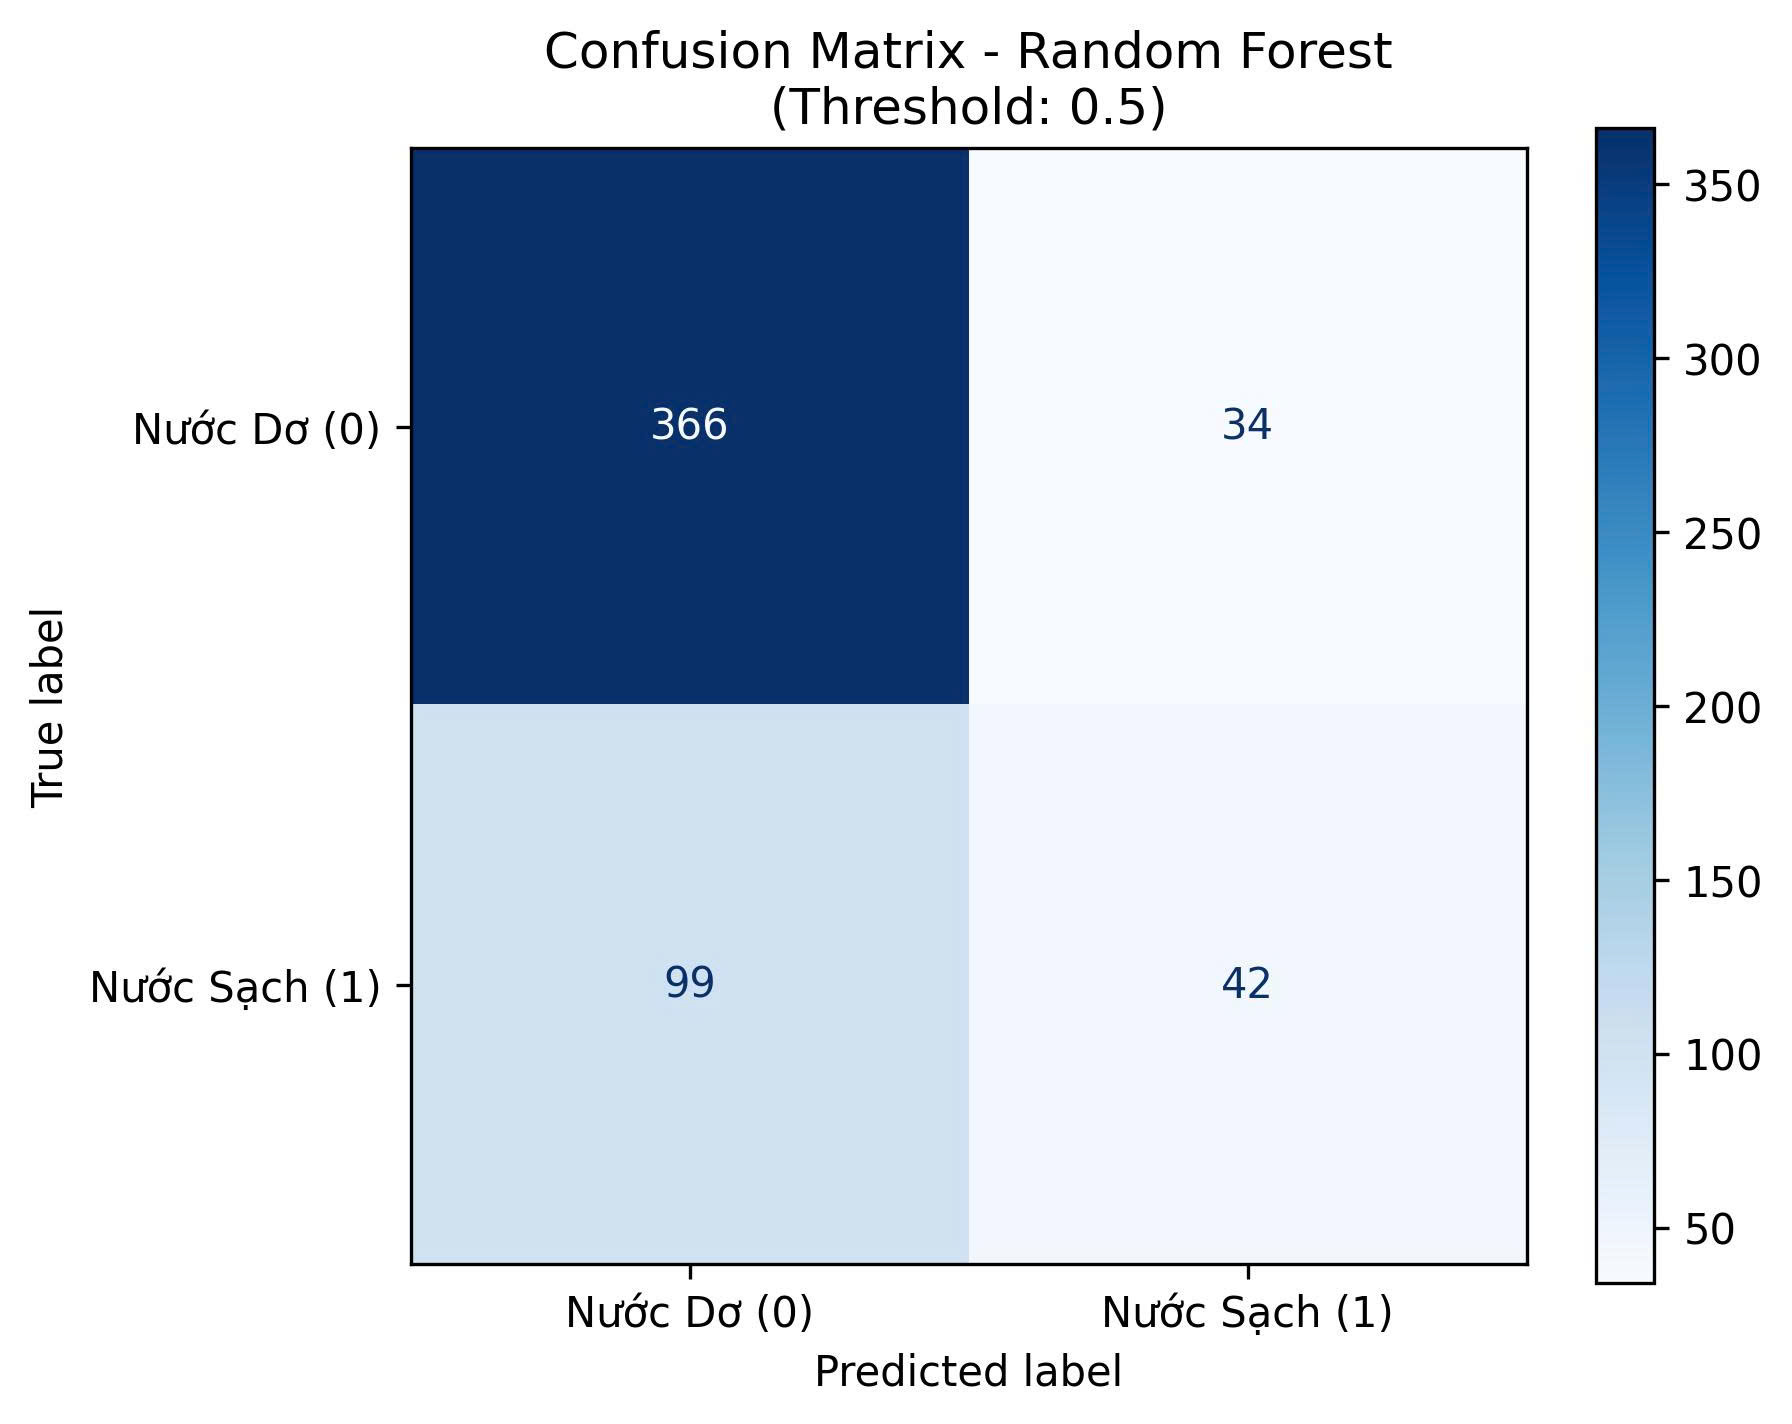
\includegraphics[width=0.6\textwidth]{IMAGE-MODELS/ConfusionMatrix_RandomForest.jpg}
    \caption{Confusion Matrix của mô hình Random Forest tại ngưỡng 0.5}
    \label{fig:cm_rf}
\end{figure}

\subsubsection{Giải thuật XGBoost (Extreme Gradient Boosting)}
\begin{table}[H]
    \centering
    \renewcommand{\arraystretch}{1.2}
    \begin{tabular}{ccccc}
        \hline
        \textbf{Threshold} & \textbf{Precision} & \textbf{Recall} & \textbf{F1-Score} & \textbf{Accuracy} \\
        \hline
        \color{red}0.50 &\color{red} 0.8182 &\color{red} 0.0638 &\color{red} 0.1184 &\color{red} 0.7523 \\

        0.55 & 1.0000 & 0.0426 & 0.0816 & 0.7505 \\

        0.60 & 0.0000 & 0.0000 & 0.0000 & 0.7394 \\

        0.65 & 0.0000 & 0.0000 & 0.0000 & 0.7394 \\

        0.70 & 0.0000 & 0.0000 & 0.0000 & 0.7394 \\

        0.75 & 0.0000 & 0.0000 & 0.0000 & 0.7394 \\

        0.80 & 0.0000 & 0.0000 & 0.0000 & 0.7394 \\
        \hline
    \end{tabular}
    \caption{Kết quả đo lường hiệu suất của mô hình XGBoost qua các ngưỡng}
    \label{tab:xgb_metrics}
\end{table}
Đối với XGBoost, tổ hợp tham số tốt nhất được hệ thống lựa chọn là: \texttt{learning\_rate=0.01}, \texttt{n\_estimators=100}, \texttt{max\_depth=7}, và \texttt{subsample=0.9}. 

Kết quả thực nghiệm cho thấy XGBoost có hành vi phân lớp khá cực đoan. Tại ngưỡng $0.5$, mô hình đạt Precision rất cao lên tới $0.8182$, tuy nhiên chỉ số Recall lại rớt xuống mức cực thấp là $0.0638$ (F1-Score chỉ đạt $0.1184$). Điều này phản ánh việc XGBoost dự đoán vô cùng "thận trọng": nó hiếm khi gán nhãn một mẫu nước là an toàn (1), nhưng một khi đã gán thì tỷ lệ đúng là rất cao. Dù Accuracy vẫn ở mức $75.23\%$, khả năng phát hiện các mẫu nước sạch của XGBoost thực tế bị hạn chế nghiêm trọng.

\begin{figure}[H]
    \centering
    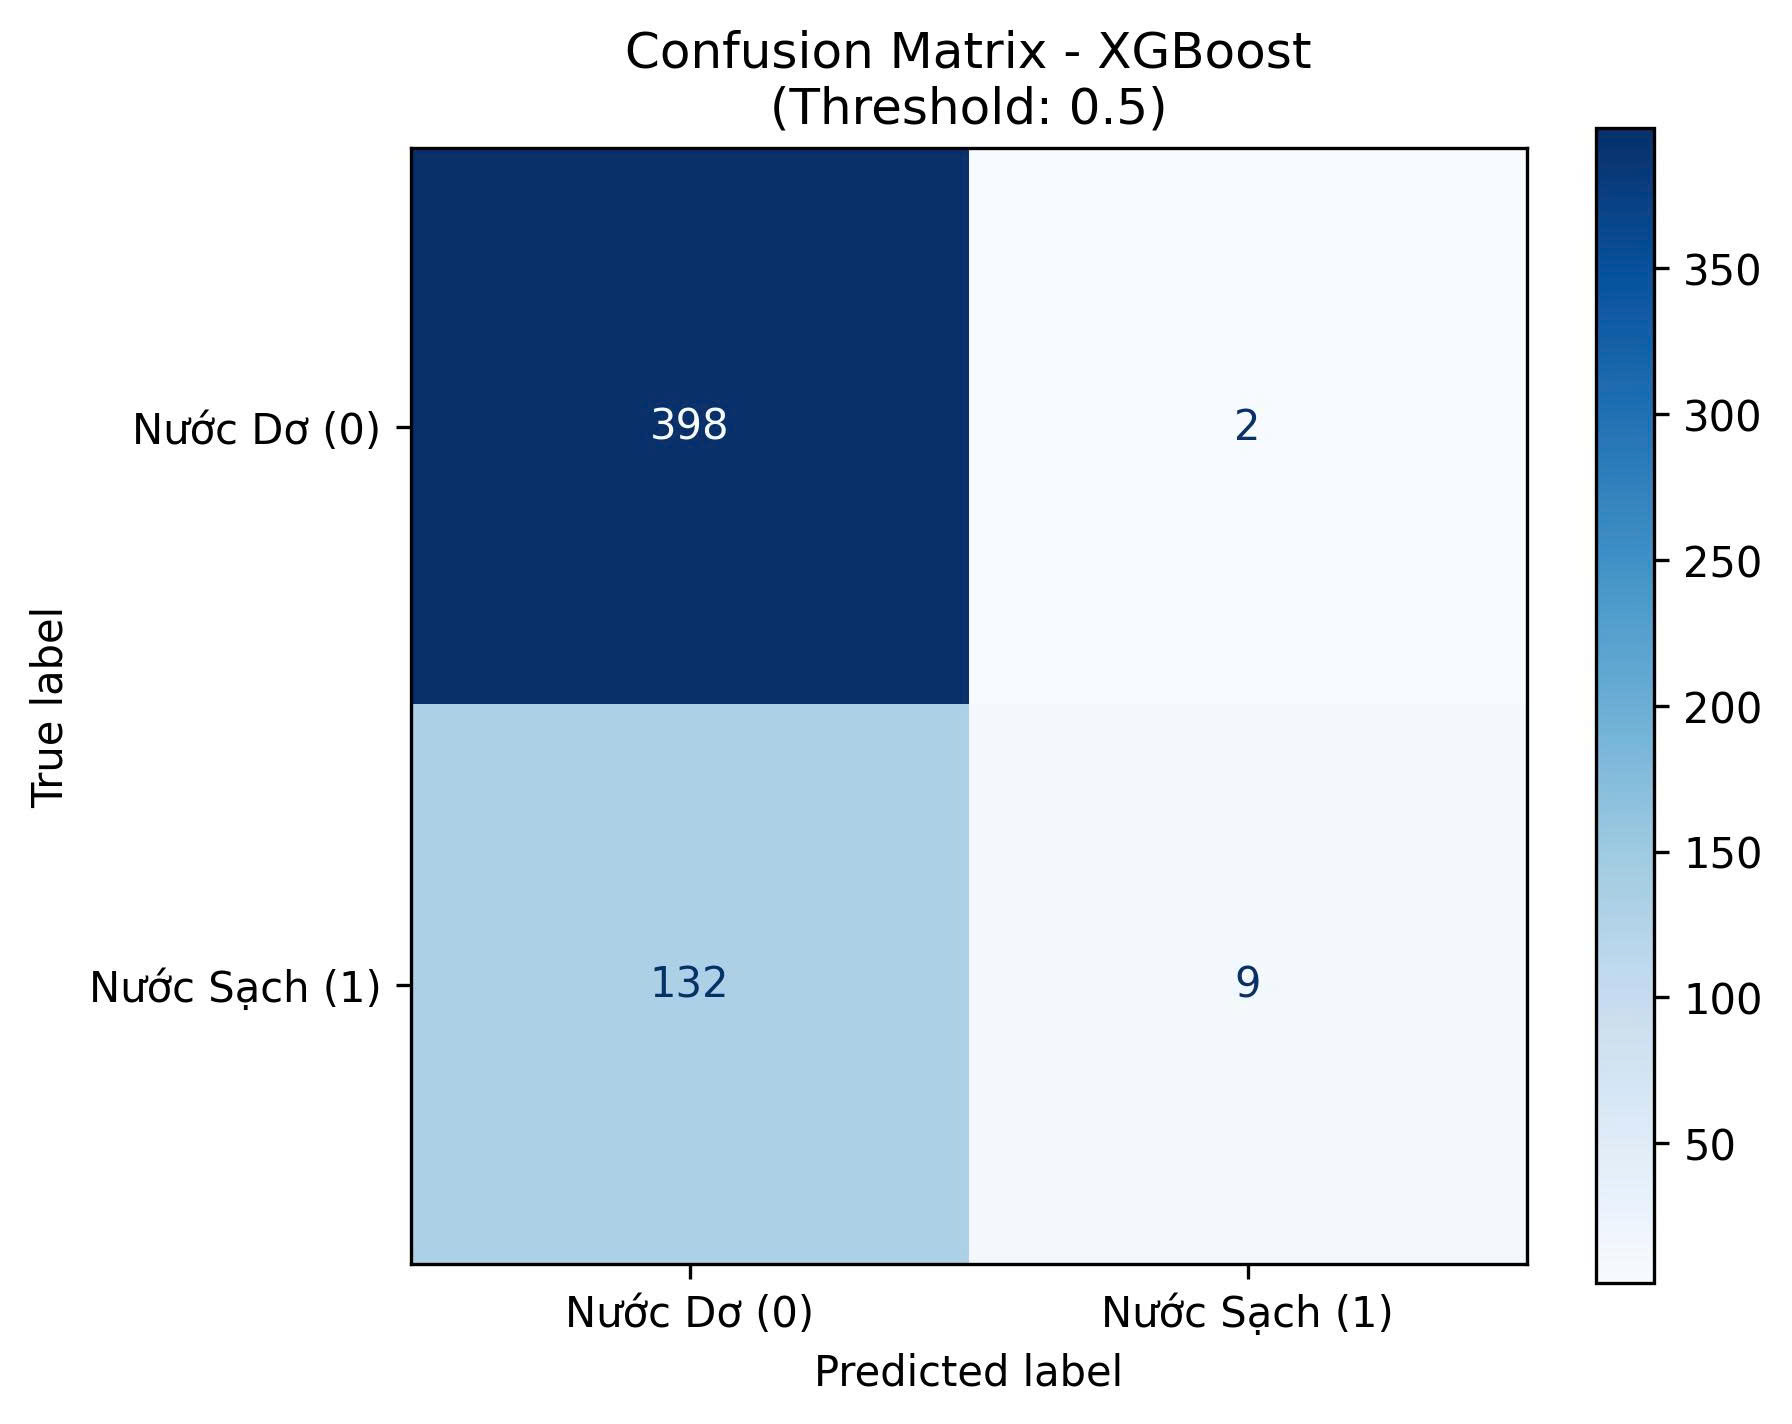
\includegraphics[width=0.6\textwidth]{IMAGE-MODELS/ConfusionMatrix_XGBoost.jpg}
    \caption{Confusion Matrix của mô hình XGBoost tại ngưỡng 0.5}
    \label{fig:cm_xgb}
\end{figure}

\subsubsection{Giải thuật Support Vector Machine (SVM)}
\begin{table}[H]
    \centering
    \renewcommand{\arraystretch}{1.2}
    \begin{tabular}{ccccc}
        \hline
        \textbf{Threshold} & \textbf{Precision} & \textbf{Recall} & \textbf{F1-Score} & \textbf{Accuracy} \\
        \hline
        \color{red}0.50 &\color{red} 0.5345 &\color{red} 0.2199 &\color{red} 0.3116 &\color{red} 0.7468 \\

        0.55 & 0.6080 & 0.1915 & 0.2903 & 0.7568 \\

        0.60 & 0.6410 & 0.1773 & 0.2770 & 0.7597 \\

        0.65 & 0.6471 & 0.1560 & 0.2514 & 0.7579 \\

        0.70 & 0.6097 & 0.1418 & 0.2353 & 0.7597 \\

        0.75 & 0.6900 & 0.1206 & 0.2040 & 0.7560 \\

        0.80 & 0.7500 & 0.0993 & 0.1758 & 0.7560 \\
        \hline
    \end{tabular}
    \caption{Kết quả đo lường hiệu suất của mô hình SVM qua các ngưỡng}
    \label{tab:svm_metrics}
\end{table}
Mô hình SVM được huấn luyện sử dụng nhân RBF phi tuyến trên tập dữ liệu đã qua tiền xử lý chuẩn hóa (\texttt{StandardScaler}). Tại ngưỡng $0.5$, SVM ghi nhận độ chính xác tổng thể (Accuracy) đạt $74.68\%$. Chỉ số Precision ghi nhận ở mức $0.5345$ và Recall là $0.2199$, cho F1-Score tương ứng là $0.3116$.

\begin{figure}[H]
    \centering
    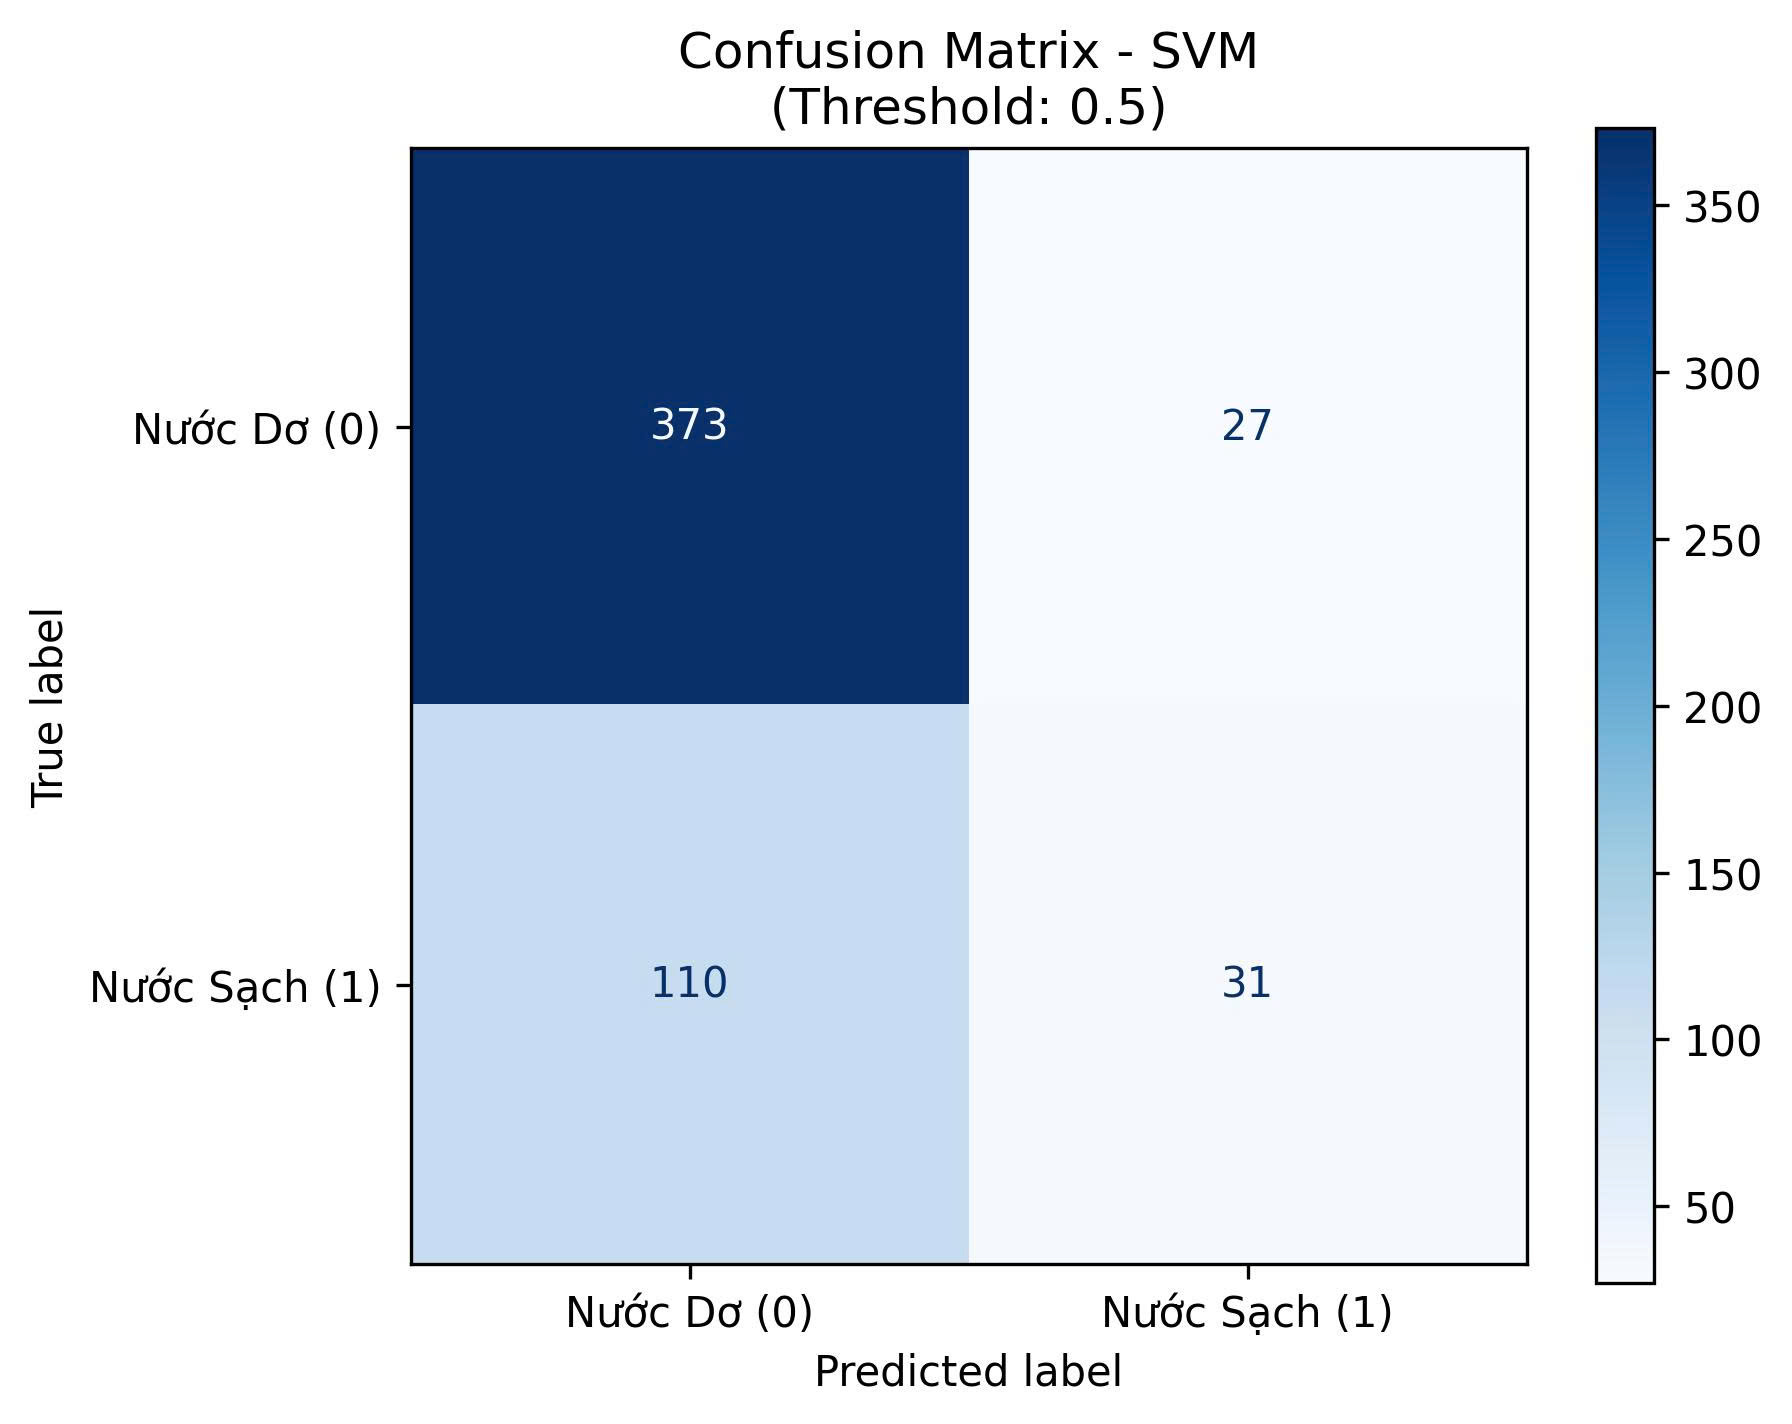
\includegraphics[width=0.6\textwidth]{IMAGE-MODELS/ConfusionMatrix_SVM.jpg}
    \caption{Confusion Matrix của mô hình SVM tại ngưỡng 0.5}
    \label{fig:cm_svm}
\end{figure}

\subsection{Đánh giá tổng quan và lựa chọn mô hình triển khai}

Từ các kết quả đo lường trên, có thể thấy Random Forest và Support Vector Machine (SVM) có hiệu suất phân lớp tương đương nhau (Accuracy đều xoay quanh mốc $75\%$). Tuy nhiên, xét trên bức tranh tổng thể về kỹ thuật và khả năng ứng dụng thực tế, nhóm quyết định lựa chọn Random Forest làm mô hình chính thức để đóng gói và triển khai. Quyết định này được củng cố bởi các luận điểm cốt lõi sau:

\begin{itemize}
    \item \textbf{Hiệu suất cân bằng (F1-Score):} Bài toán có sự chênh lệch dữ liệu dẫn đến việc Accuracy không phản ánh được toàn bộ vấn đề. Xét trên F1-Score (thước đo dung hòa giữa Precision và Recall), Random Forest ($0.3871$) thể hiện khả năng nhận diện nguồn nước sạch nhỉnh hơn hẳn so với SVM ($0.3116$).
    
    \item \textbf{Tối ưu chi phí tiền xử lý (Preprocessing Overhead):} Thuật toán SVM cực kỳ nhạy cảm với thang đo của dữ liệu, bắt buộc hệ thống phải trải qua bước \texttt{StandardScaler} để đưa các đặc trưng về cùng một phân phối. Ngược lại, Random Forest là thuật toán dựa trên phân chia nhánh cây (Tree-based), hoàn toàn "miễn nhiễm" với sự chênh lệch đơn vị đo lường. Lựa chọn Random Forest giúp hệ thống rút ngắn được một khâu tiền xử lý, tăng tốc độ dự đoán (Inference time) khi triển khai luồng dữ liệu thực tế.
    
    \item \textbf{Tối ưu hóa không gian lưu trữ và bộ nhớ (Model Size \& Memory):} Quá trình dự đoán của SVM đòi hỏi phải lưu trữ lại rất nhiều điểm Vector Hỗ trợ (Support Vectors) từ tập huấn luyện. Với một bộ dữ liệu phân tán phức tạp như tính chất hóa lý của nước, file lưu trữ \texttt{.pkl} của SVM thường bị "phình to" về mặt dung lượng. Hơn nữa, để đưa lên môi trường sản phẩm (Production), hệ thống phải tải cùng lúc cả file \texttt{Scaler.pkl} và \texttt{Model.pkl}. Trái lại, Random Forest chỉ cần một tệp trọng số duy nhất, cấu trúc gọn nhẹ, ít tiêu tốn tài nguyên RAM của máy chủ lưu trữ (Server), đáp ứng hoàn hảo tiêu chí của một ứng dụng dự đoán nhanh.
\end{itemize}